\documentclass{article}
\usepackage[margin=1.0in]{geometry}

\usepackage{amsmath}
\usepackage{amsfonts}
\usepackage{amssymb}
\usepackage{graphicx}
\usepackage[hidelinks]{hyperref}
\usepackage{lineno}
\usepackage{booktabs}

\usepackage{graphicx}
\usepackage{caption}
\usepackage{subcaption}
\usepackage{hyperref}

\usepackage{listings}
\usepackage{xcolor}

\colorlet{punct}{red!60!black}
\definecolor{background}{HTML}{EEEEEE}
\definecolor{delim}{RGB}{20,105,176}
\colorlet{numb}{magenta!60!black}

\lstdefinelanguage{json}{
    basicstyle=\normalfont\ttfamily,
    numbersep=8pt,
    showstringspaces=false,
    breaklines=true,
    literate=
     *{0}{{{\color{numb}0}}}{1}
      {1}{{{\color{numb}1}}}{1}
      {2}{{{\color{numb}2}}}{1}
      {3}{{{\color{numb}3}}}{1}
      {4}{{{\color{numb}4}}}{1}
      {5}{{{\color{numb}5}}}{1}
      {6}{{{\color{numb}6}}}{1}
      {7}{{{\color{numb}7}}}{1}
      {8}{{{\color{numb}8}}}{1}
      {9}{{{\color{numb}9}}}{1}
      {:}{{{\color{punct}{:}}}}{1}
      {,}{{{\color{punct}{,}}}}{1}
      {\{}{{{\color{delim}{\{}}}}{1}
      {\}}{{{\color{delim}{\}}}}}{1}
      %{[}{{{\color{delim}{[}}}}{1}
      %{]}{{{\color{delim}{]}}}}{1},
}

\linenumbers

\newcommand{\median}{\operatorname{median}}

% http://bytesizebio.net/2013/03/11/adding-supplementary-tables-and-figures-in-latex/
\newcommand{\beginsupplement}{%
        \setcounter{table}{0}
        \renewcommand{\thetable}{S\arabic{table}}%
        \setcounter{figure}{0}
        \renewcommand{\thefigure}{S\arabic{figure}}%
     }

\hyphenation{Ge-nome Ge-nomes hyper-mut-ation through-put}

\title{Phippery: A phage immunoprecipitation sequencing pipeline to characterize antibody targets}
\author{Jared G. Galloway}

% QUESTION: Where should we squeeze in phage-dms explanation? discussion?

\begin{document}
\maketitle

\begin{abstract}
A globalized world has drafted more urgency and attention to the danger of pathogens.
With this sentiment, the vast community of research in this realm have proliferated the effectiveness of our own immune system to combat disease.
The adaptive immune system interacts with and identifies pathogens by complex mechanisms of cell digestion, selection and mutation --
a process which produces molecular locks on specialized cells, most commonly, antibodies.
The pathogen's surface proteins act as a key, and are thus flagged to be destroyed when the complimentary antibody cells bind.
Identifying both the binding specificities of sample antibody repertoires (usually from blood serum), as well as the knowing the key for pathogens of interest remains an outstanding and challenging problem in serology. 
Addressing these questions, a method known as Phage Immuno-Precipitation Sequencing, or \textbf{PhIP-Seq}, has presented itself as a promising protocol for investigation of antibody targets.
This method allows us to observe and quantify the protein-protein interactions between a set of antibodies and artificial epitopes displayed on phages (phage vectors).
By designing and synthesizing phages displayed proteins, researchers can model the span of potential epitopes encoded by any locus in a pathogen's genome.
The protocol ultimately results in an \textit{enrichment} matrix where each entry represents the number of peptide-antibody binding events observed when serum is exposed to the phage library.
Notably, this protocol requires clever experimental design, sensitive wet-lab technique, a bioinformatics pipeline, and powerful statistical tools to parse signal from various sources of noise.
In this paper, we will present computational tools to help deal with the bioinformatics, and book-keeping as well as set the stage for analysis by providing a well-defined data structure to organize the entire dataset.
Specifically, we provide a \textbf{Nextflow} analysis pipeline that takes in demultiplexed next generation sequencing files and produces a coherent dataset to be queried
Finally, we present some figures produced by running the pipeline with an anonymous, empirical dataset focused on SARS-CoV-2.
\end{abstract}

\section*{Introduction}

The immune system is most simply divided into two biological mechanisms which we call the \textit{innate} and \textit{adaptive} immune systems \cite{Jain2017}.
The \textit{innate} immune system is primarily made of informed by cells, such as leukocytes, which classify an object as either foreign or native to the body.
When a foreign object is detected, the body immediately responds with a set of non-specific deterrents such as inducing a fever.
If the pathogen survives these initial defence mechanisms, the body's second wave of defence is a more targeted attack known as the adaptive immune response.
The relies upon generating antibodies which can identify a singular pathogen which induced the response. 
Antibodies primary job is to ``tag" a pathogen which can then signal a specialized cell, such as a natural killer cell (NKC) to destroy it later. 
The ability to rapidly respond to the same pathogen after the initial infection is known as \textit{immunity} and it is a product of the adaptive immune system ``memory".
When designing a vaccine for a specific virus, the memory of the adaptive immune system is leveraged by provoking the immune response with a 
neutralized representation of the virus.
This needs to be similar enough to the real virus that it allows the body to generate the right cell machinery, without exposing the individual to a dangerous pathogen.
It follows that knowledge of antibody binding specificities would inform a great deal about the natural defences, or lack of, an individual possesses.
Further, identification of the molecular key, often referred to as the \textit{epitope}, as the primary identifier of a specific pathogen to an antibody could greatly simplify the process of vaccine design.
Obtaining this information remains an outstanding challenge in the field of serology, but several advances have recently been made to help us investigate \cite{Doepker2020}.

For linear epitopes, we know that the oligonucleotide sequence encoding for this protein lives somewhere where in the genome of the pathogen.
By synthesizing the span of potential epitope-encoding nucleotides across the exon's of a pathogen genome,
researchers can leverage Next Generation Sequencing (NGS) to quantify the binding specificities of sample antibodies \cite{Jody2010, Khan2020}. 
This is a novel technique known as Phage Immuno-Precipitation Sequencing, or \textbf{PhIP-Seq} \cite{Larman2011}.
The PhIP-Seq protocol first requires that a researcher design a peptide library from a set of pathogen genome loci of interest.
The libraries are most commonly generated using a sliding window across a locus producing oligonucleotide ``tiles" encoding for a peptide.
The size and stride of the nucleotide tiles is designed using specialized software before they are synthesized.
These nucleotide chains are then cloned into a phage with the hope that it models the potential molecular key on the surface of a pathogen. 
When mixed with antibodies, phages that have bound with an antibody are ``precipitated" out of the mixture using magnetic beads with a technique referred to as Immuno-Precipitation (IP).
The key idea being that the repertoire of phages caught on the beads should then be representative of antibody targets from the sample.
The samples themselves can come from a variety of sources and individuals most fitting to the experiment being run. 
It should be noted that in nature, we expect the ``epitope" of any particular pathogen to be either \textit{linear} or \textit{conformational}.
Conformational epitopes are proteins which have a \textit{tertiary} structure, meaning the protein has folded and the epitope can no longer be represented by the linear chain of nucleotides encoding for the protein.
The nature of this protocol means that we can only identify \textit{linear} epitopes as the phage-displayed peptides are sequential in practice.

After the IP step as been performed,
researchers can then quantify the number of phages caught on the beads using barcoded short-read alignment. 
From a broad perspective, the analysis of these data consists primarily of demultiplexing the samples,
then aligning the peptides to the reference library.
By computing the number of read hits for a specific peptide sequence, we generate a count of each specific peptide and sample binding event observed. 
The final result is in the form of a matrix, $X$, where (heuristically) there is a row, $i$, for each peptide and a column, $j$, for each sample.
Concretely, $X_{j,i} =$ the number of reads from sample $i$, which contain the peptide $j$.

Doing analysis for this protocol presents two challenges:
(1) This protocol requires an immense amount of book-keeping and computational power to produce coherent results.
(2) From this protocol, there are a variety of sources we can expect add noise to the resulting data, these are including but not limited to; 
IgG content of a sample, "immuno-dominant" antibodies, sequencing bias, amplification bias, and phage display (total amount of each phage in the phage library) \cite{Yuan2018}. 
Here, approach the first problem by presenting and describing a novel \textbf{Nextflow} pipeline constructed to handle all bookkeeping and data processing steps in parallel \cite{DiTommaso2017}.
The pipeline shows promising results and -- when tested on an empirical dataset focused on SARS-CoV-2 -- completes over $900$ data processing steps in less than ten minutes.
Additionally, we provide some preliminary results analyzing the output from this pipeline using a python package, \textbf{phippery}, specifically designed for the organization and inspection of the pipeline output.

\section*{Methods}

In data science, a pipeline is loosely defined set of data processing steps to be run in sequence. 
Pipeline managers such as \textbf{Snakemake} and \textbf{Nextflow} compile the dependencies of one process to the next based on the input \cite{Merkel_2017, Koster2012}.
Ultimately this results in a Directed Acyclic Graph (DAG) of data processing steps and their respective execution order. 
In the context of PhIP-Seq, the nature of many seperate sample alignments to different peptide-encoding nucleotide sequence references makes this workflow a perfect candidate for a workflow manager which can perform these steps in parallel on a high performance computer (HPC). 
For this specific pipeline we use Nextflow paired specialized docker containers to produce a reproducible and highly-parallelized workflow.

Nextflow is primarily defined by a set of \textit{Processes}, \textit{Channels}, and \textit{Operators}.
Each process block defines a singular data processing step, given some inputs, using either a command line script or one of a few popular data-driven scripting languages.
Each process execution is run in a containerized environment where the inputs are staged in an independent temporary directory making it autonomous to the rest of the pipeline execution steps.
The pipeline manager handles all process inputs and outputs through \textit{Channels} so the individual processes don't conflict with each other in terms of file system or necessary software dependencies.
A \textit{Channel} can be thought of as a First-In-First-Out (FIFO) queue and acts as the only mode of communication between the data processing steps.
Processes which define their input from a channel are executed as soon as something is put in the queue.
\textit{Operators} allow us to merge, split, or transform the items placed in a channel to configure a nicely formatted output usually containing files and metadata
needed for a downstream process.
Figure \ref{fig:DAG} shows the DAG of our pipeline from input metadata and sequencing file to a specialized python object containing
the respective counts and metadata for each sample and peptide \cite{van1995python}.
In this section, we will discuss the pipeline inputs, the individual steps of the pipeline, and the resulting output.

\begin{figure}[h!!!!]
\centering
    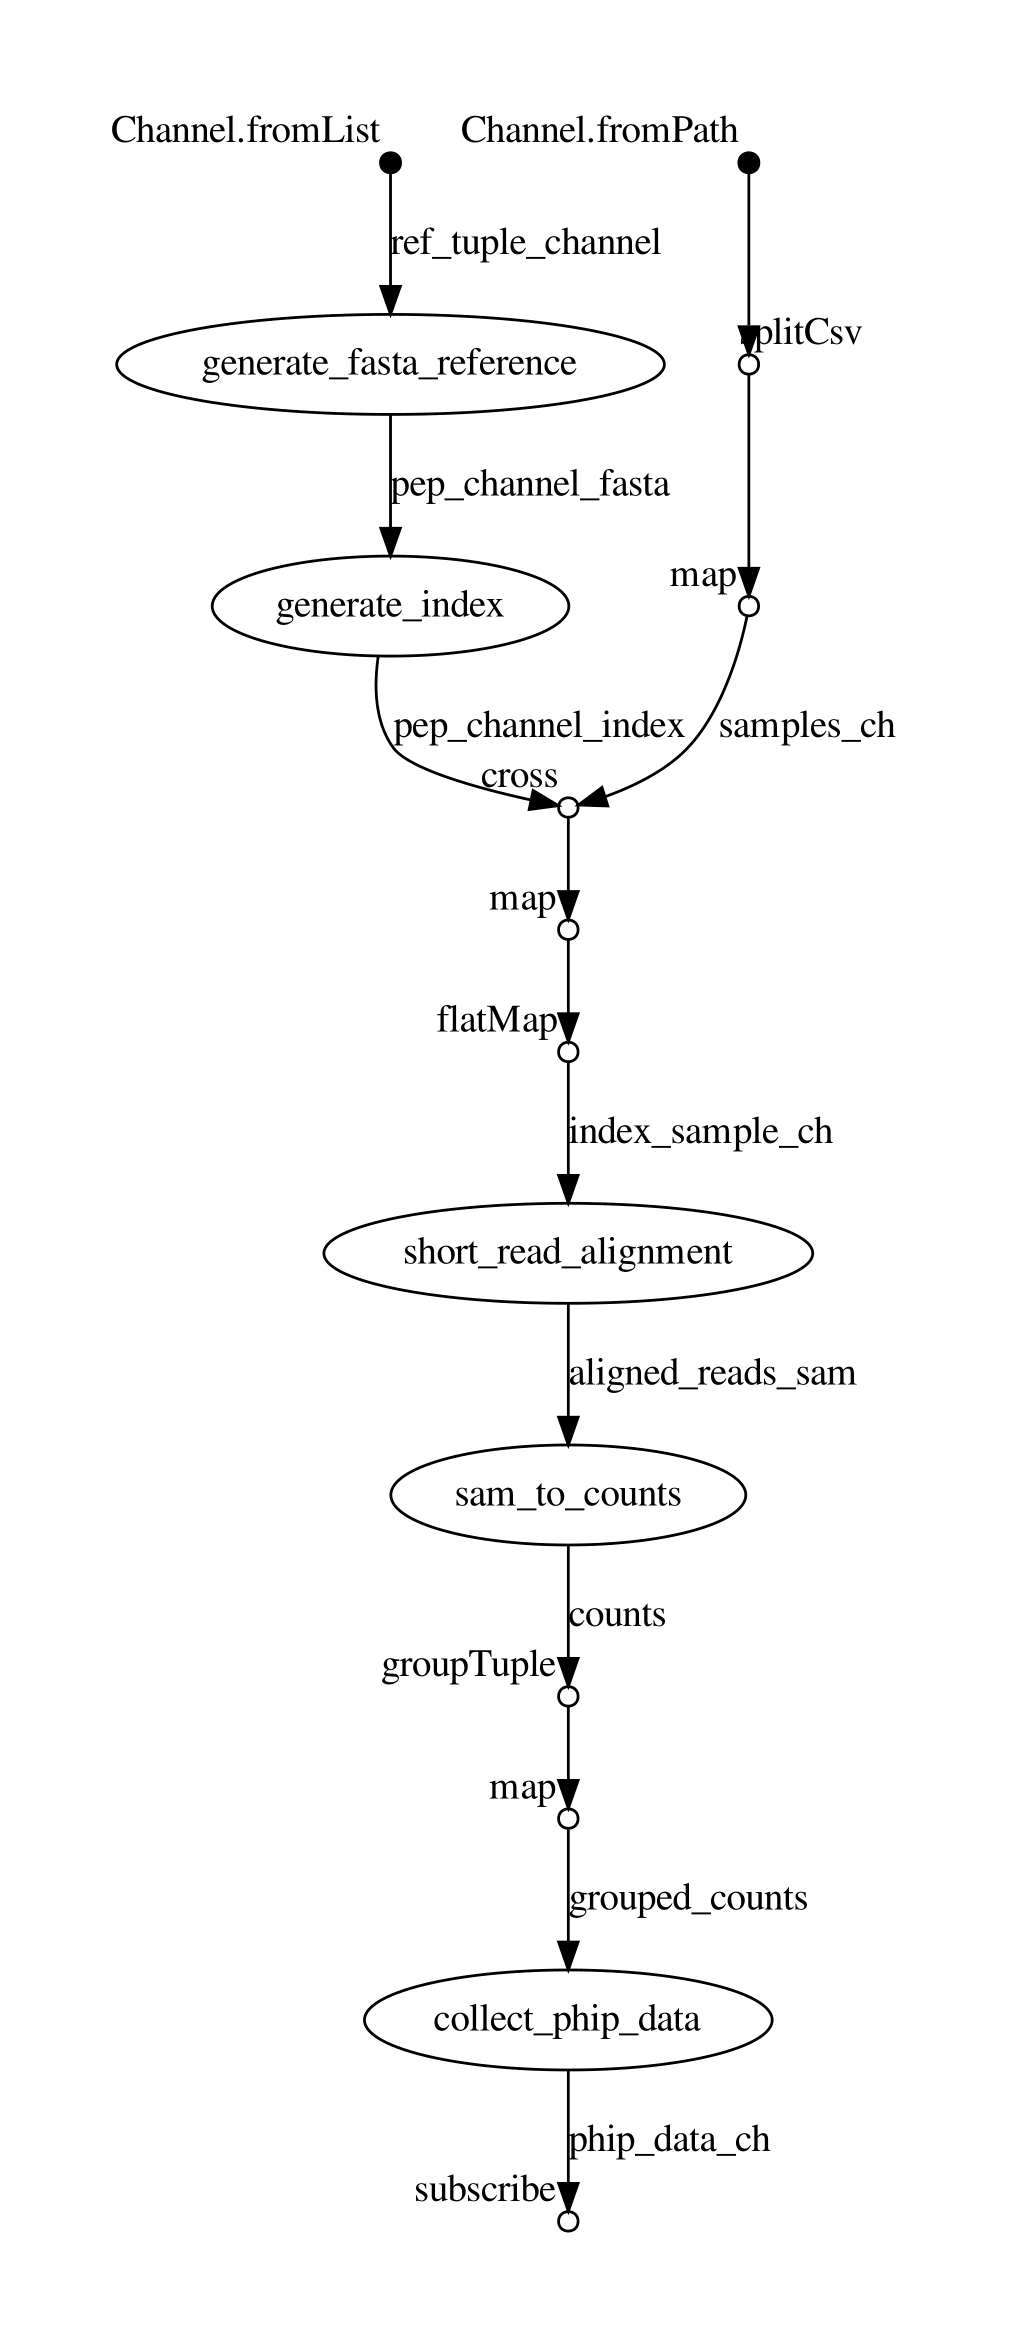
\includegraphics[width=0.5\textwidth]{figures/dag-1.png}
    \caption { \
The Directed Acyclic Graph (DAG) representation of our pipeline workflow. 
Here, each bubble represents a single data processing step to be run in temporary directory inside a respective docker container. 
The arrows specify \textbf{Nextflow} ``channels" which direct and organize output from one process to the next. 
Dots between channel arrows specify where a \textbf{Nextflow} ``operator" was used to organize and collect the output of a set of channels into another set of channels.
}
\label{fig:DAG}
\end{figure}

\subsection*{Pipeline Input - Data}

To configure the run of a pipeline the user must specify the path of JSON configuration file.
This file contains information about where the pipeline can find sample and peptide metadata, 
the sample fastq files for each experiment, and lastly, some information about read and reference nucleotide length. 
Using this, the pipeline automatically parses the JSON file and configures the steps needed to generate the output.
This approach allows the user to organize their data how they like, and let the pipeline manager structure pipeline output..

\paragraph{Configuration file}
There a few key-value pairs that are required to be in the configuration file. 
An example configuration file for a simulated dataset is shown in Listing \ref{listing:config.json}.
First the user must specify an ``output\_dir" key with the value as a file path where the would like the results of the pipeline to be published.
The ``samples" key must specify a valid path to a sample metadata csv described below. 
Each sample is tied directly to one of the keys specified in ``experiments", 
thus, the path to the base directory holding all sample files must be specified for \textit{each} experiment.
Similarly, each sample specifies a reference library it should be aligned against, this is the ``reference" column.
Additionally, there are a few other parameters which can be used to specify read and reference oligo length for alignment schemes.
It should be clear that only a \textit{single} sample metadata csv is specified, while \textit{multiple} peptide references can be specified.
The pipeline will output a phippery PhipData object for each reference containing the respective samples as described in the sample metadata file.

\begin{lstlisting}[language=json,firstnumber=1,caption={An example JSON configuration file for a simulated dataset.},captionpos=b,numbers=none,label=listing:config.json]
{
    "output_dir" : "simulate_ones/",

    "samples" : "simulate_ones/samples/sample_metadata.csv",

    "experiments" : {
        "expa" : "simulate_ones/experiments/expa/some/path/",
        "expb" : "simulate_ones/experiments/expb/some/path/"
    },

    "references" : {
        "refa" : "simulate_ones/references/peptide_metadata_a.csv",
        "refb" : "simulate_ones/references/peptide_metadata_b.csv"
    }
}
\end{lstlisting}

\paragraph{Sample metadata}
To specify which samples are included in the pipeline run, 
the researcher who designs the experiment compiles a comma-separated file specifying all relevant metadata for each Immuno-Precipitation experiment run. 
Table \ref{tab:sample_metadata} shows an example of this sample metadata table for simulated data.
There are four required fields that must be specified for each sample (row) in the file;
(1) A unique identifier in the form of a single integer, specified in the ``ID" column.
(2) The file \textit{pattern} which specifies the filenames for all technical replicates of a single sample in the ``fastq\_pattern" column.
(3) An ``experiment" name which, in the config file, ties the sample to the location of the base directory where the fastq file is expected to be found.
(4) A ``reference" name which specifies the index the samples should be aligned to.
While this presents only \textit{required} fields, it's generally useful to add any other relevant metadata connected to each sample such as sample type, species etc.
Any and all fields can be used for downstream analysis when querying the dataset. 

\begin{table}[h!!!!]
\centering
\begin{tabular}{llll}
\toprule
{} &           fastq\_pattern & reference & experiment \\
ID &                         &           &            \\
\midrule
0  &              sample-*-0 &      refa &       expa \\
1  &              sample-*-1 &      refa &       expa \\
2  &  xeno-AE-122-*-R1.3.3.0 &      refa &       expa \\
3  &  xeno-AE-122-*-R1.3.3.1 &      refa &       expa \\
4  &  xeno-AE-122-*-R1.3.3.2 &      refa &       expa \\
5  &  xeno-AE-122-*-R1.3.3.3 &      refb &       expb \\
6  &  xeno-AE-122-*-R1.3.3.4 &      refb &       expb \\
7  &          johnny-boy-*-0 &      refb &       expb \\
8  &          johnny-boy-*-1 &      refb &       expb \\
9  &          johnny-boy-*-2 &      refb &       expb \\
\bottomrule
\end{tabular}
\caption{An example sample metadata table containing the requires fields for a simulated dataset.}
\label{tab:sample_metadata}
\end{table}

\paragraph{Peptide metadata}
For each unique reference listed in sample metadata file, we must specify a peptide metadata comma-separated file in order to build an index. 
As seen in Table \ref{tab:peptide_metadata}, there only two required fields;
(1) A unique identifier in the form of a single integer, specified in the ``ID" column.
(2) the ``Oligo" column specifying the nucleotide encoding for a specific peptide. 
Currently, we expect the index oligo sequences, if there at all, be lowercase and the peptide encoding sequence be uppercase.
Similarly to the sample metadata table, it is generally useful to include other information about the peptide such the virus
strain, and some genomic positional information.

\begin{table}[h!!]
\centering
\begin{tabular}{ll}
\toprule
{} &                                              Oligo \\
ID &                                                    \\
\midrule
0  &  gcatcagtaggctgcgtaGGGATTAGGCGGACCTCCATGAATACCG... \\
1  &  gcatcagtaggctgcgtaTGTAGGCAAGGAGCAACACTTCTTCTTT... \\
2  &  gcatcagtaggctgcgtaGAGAATGGGCCAGGAATGATCTACTGTC... \\
3  &  gcatcagtaggctgcgtaCGTGTCAAAAACTGCGTATTTACGAAGA... \\
4  &  gcatcagtaggctgcgtaTTTCAGATCCTACCATTTGTGTCCTTAA... \\
5  &  gcatcagtaggctgcgtaCCGAGTTCGTATTTTTACAAATCCCGGA... \\
6  &  gcatcagtaggctgcgtaTATTTAATGAGTGTGAGGCAAAGTTGTT... \\
7  &  gcatcagtaggctgcgtaTTTACGCTCAGCAAGCGTAGCTAGCATG... \\
8  &  gcatcagtaggctgcgtaTCAAACAGGTTACGACACAAAGAACGCC... \\
9  &  gcatcagtaggctgcgtaTCGCATTCTCCTGGCCTACTTACAGTTC... \\
\bottomrule
\end{tabular}
\caption{An example peptide metadata table containing the requires fields for a simulated dataset.}
\label{tab:peptide_metadata}
\end{table}

\subsection*{Data Processing Steps}

There are a number of individual data processing steps that take place when running this pipeline.
The number of times each process is run is determined by the number of references and samples.
Concretely, if there are $S$ samples, each with $T$ technical replicates and $R$ references, then we can expect $2ST + 3R$ separate processes to be run. 
In this section, we will briefly review the unique data processing steps in the pipeline.
The pipeline begins by defining two input channels; 
the first channel defines the references to be generated and their respective peptide metadata tables,
the second channel parses each sample in the sample metadata file, finds all technical replicates for that sample, and merges with the first channel.
In short, the pipeline the performs sequence
alignment, counts generation, and counts merging.

\paragraph{generate fasta reference}
The first step in the pipeline is to parse the configuration file for all listed references and respective peptide metadata files. 
For each reference found, the pipeline executes a ``generate\_fasta\_reference" process.
The primary job for this step is to produce a fasta representation of the respective peptide metadata table in preparation for index generation.
Simply put, this step simply converts the ID into a header followed by the nucleotide sequence encoding for each peptide in the table.
A container for the \textbf{phippery} python package is used as the primary execution step.
For cluster submission, we request only a single core with a modest amount of memory because the software being used isn't multithreaded.

\paragraph{Index generation}
For samples to be aligned to the reference, a specific binary index must be generated.
In this step, we use \textbf{bowtie-build} to generate the index which each respective sample will be aligned to \cite{Langmead2009}
The five binary files that are output are nested in a subdirectory dir named ``<reference name>\_index".
This process is run in a public \textbf{bowtie} container hosted on Quay and \textit{can} be multithreaded. 

\paragraph{Short read alignment}
The bulk of the work performed in the pipeline happens during short-read sequence alignment of every technical replicate to it's respective reference peptide library.
After the references have been built and the sample metadata file has been parsed, we merge the channels into a new channel, named \textit{index\_sample\_ch}.
Taking in metadata, and reference for a single technical replicate, we perform end-to-end short read alignment using \textbf{bowtie} \cite{Langmead2009}.
Unlike most alignment scenarios, we are not looking for a read \textit{within} a reference sequence, but rather our nucleotide encoding of peptide references in a sample read.
Concretely, we trim the 3' (low-quality) end of each sample read by the difference in length between the reference and the read.
For example, if our read length is $125$bp and out peptide references tiles are $117$bp, the we trim $8$bp from the right side of the read and look and perform alignment.

~

\begin{lstlisting}[language=bash,caption={bash version}, caption={Short-read alignment parameters},captionpos=b,numbers=none,label=listing:alignment.bash]
        zcat ${respective_replicate_path} |
        bowtie --trim3 ${trim} -n ${num_mm} -l ${tile_length} \
        --tryhard --nomaqround --norc --best --sam --quiet \
        ${index}/${ref_name} - \
        > ${ID}.${replicate_number}.sam
\end{lstlisting}

~

The output from this step is a sam file named named by sample id, and technical replicate number. 
Each line in the sam file gives alignment information about the same reads.

\paragraph{alignment counting}
After the samples have been aligned, we need to compute the number of reads which aligned to each separate peptide. 
Here, we use \textbf{samtools-idxstats} tool to parse each sam file and output a two column tsv for each respective technical replicate \cite{Li2009}.
Before computing the counts, we must convert to a binary format (BAM), index, and sort the samfile to prep it for \textbf{samtools-idxstats}.

~

\begin{lstlisting}[language=bash,caption={bash version}, caption={samtools processing steps},captionpos=b,numbers=none,label=listing:samtools.bash]
        samtools view -u -@ 4 \${sam_file} | \
        samtools sort -@ 4 - > ${ID}.${replicate_number}.bam
        samtools sort -@ 4 ${ID}.${replicate_number}.bam \
        -o ${ID}.${replicate_number}.sorted 
        mv ${ID}.${replicate_number}.sorted ${ID}.${replicate_number}.bam
        samtools index -b ${ID}.${replicate_number}.bam
        samtools idxstats ${ID}.${replicate_number}.bam | \
        cut -f 1,3 | sed "/^*/d" > ${ID}.${replicate_number}.tsv
\end{lstlisting}

~

The tab-separated values file for each sample contains two columns; the first being the peptide ``ID" number, and the second is the number of alignments reported with no more than \$\{num\_mm\} mismatches as described in the alignment step.

\paragraph{merging counts and metadata}
The final step of the pipeline needs to collect \textit{all} the counts files for a single reference, and merge them into a coherent dataset.
To do this, we use custom code in \textbf{phippery} designed to merge all sample counts given a list of tsv files described in the previous step. 
First the code looks for all technical replicates of a single sample, then computes correlation and takes the mean (or optionally, the sum) of the sample before merging into the final counts table by peptide ID. 
This means that each individual sample will be presented as a single column in the counts table, and the rows will represent peptide counts. 
Finally, this step appends technical replicate info onto sample metadata and produces a \textbf{phippery.PhipData} object described in more detail below.

\subsection*{Pipeline Output}

When doing analysis on the resulting counts from an experiment, it's imperative that we have access to all metadata for each sample and peptide.
this is because the metadata defines all interesting aspects and subsets of the entire counts table.
Often, we would like to do things like; compare and contrast counts between sample groups, normalize counts by negative controls, or even look for cross reactivity between virus strains.
Ultimately, we have three tables that constitute the entirety of a dataset for a given peptide reference library;
(1) the \textit{counts} table where the peptide enrichments numbers are held for each sample,
(2) the \textit{peptide metadata} table containing things like nucleotide encoding and information about there that tile derived from, biologically, and
(3) the \textit{sample metadata} table giving a way to make sense of enrichment we see across different sample types.
The python package we created, \textbf{phippery}, centers around a python Object, \textbf{PhipData}, defined primarily by these three tables.
Additionally, it provides a useful and tested array of methods to perform set operations on the entire dataset.
The key to keeping these three tables organized and trivial to query is the fact the peptide metadata and counts share the same index columns,
and the sample metadata index matches the counts columns. 
Each of these tables are queried in together by the unique identifiers (``ID" column) specified in the metadata tables that was initially provided to the pipeline.
Figure \ref{fig:PhipData} visualizes this relationship.

\begin{figure}[h!!!!!!!]
\centering
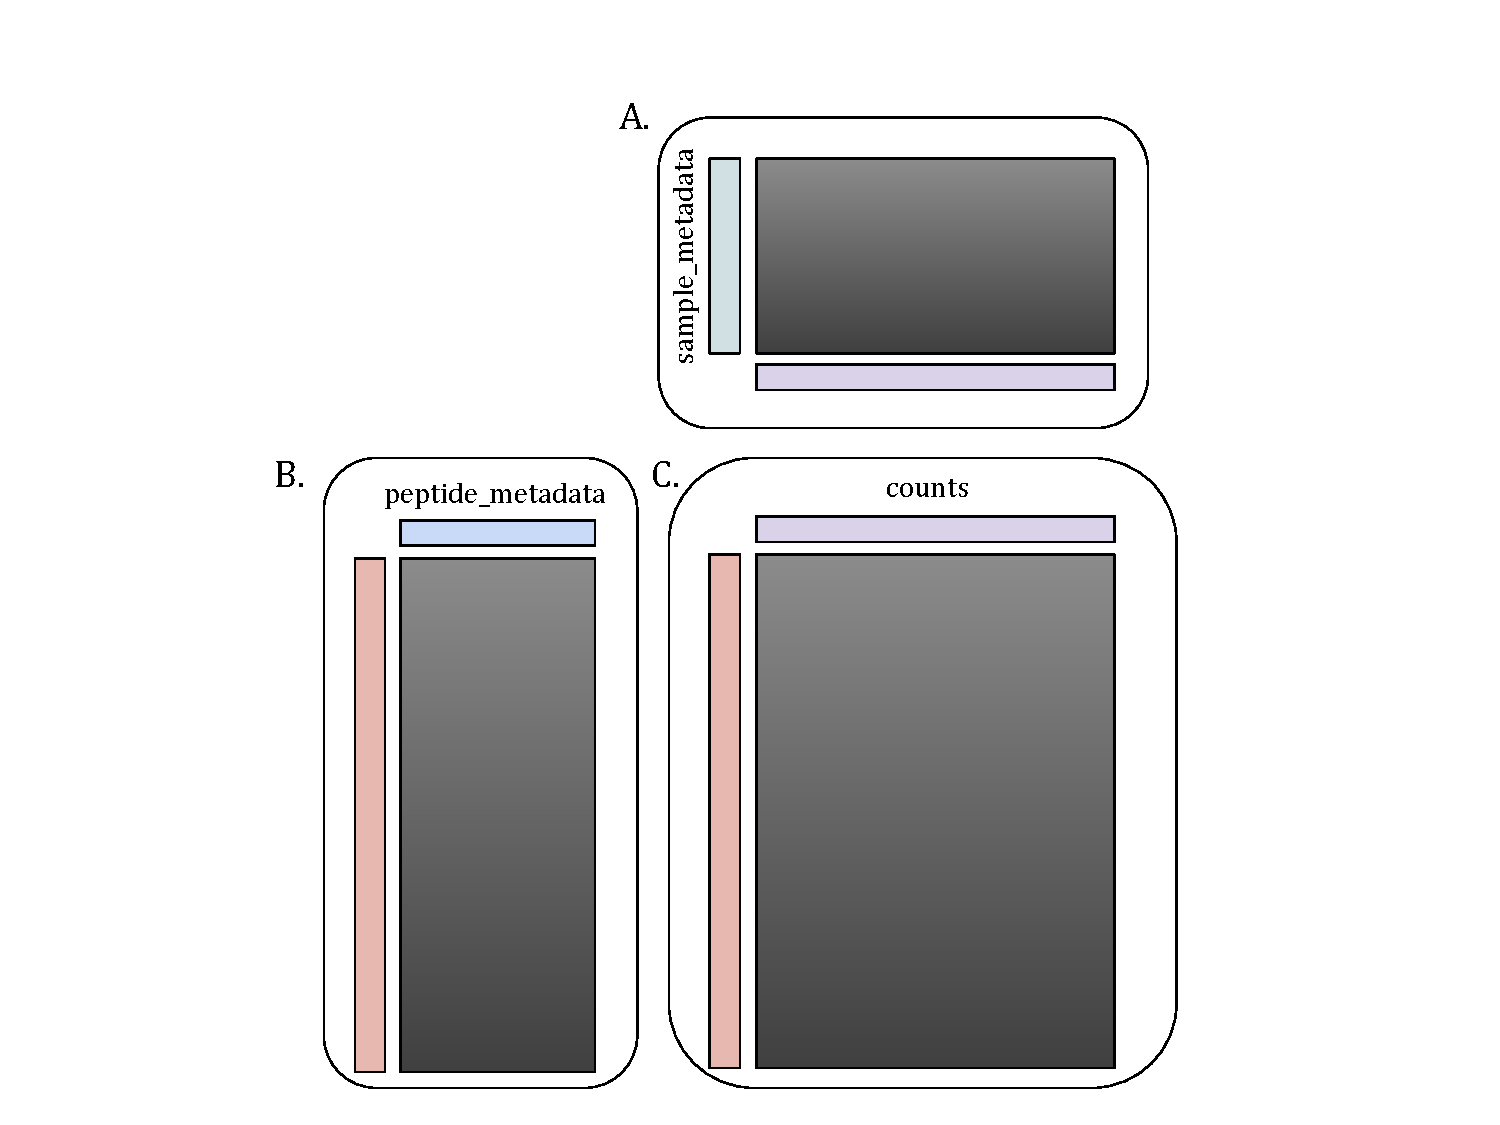
\includegraphics[width=0.60\textwidth]{figures/PhipData_Object.pdf}
\caption{ \
Cartoon of a PhipData Python Object. 
Most notably, the \textit{orange} rectangles in tables B and C represent the synchronized index for peptide metadata and
row counts. The \textit{purple} rectangles seen in A and C represent the synchronized sample metadata index with the counts column headers.
}
\label{fig:PhipData}
\end{figure}

\section*{Pipeline results on an anonymous dataset}

The pipeline described above has thus far been used on a novel set of empirical datasets focused on SARS-CoV-2.
For the purpose of example, we will include some figures produced from one of these pipeline runs.
However, due to the unpublished, private and preliminary nature of the data thus far, we will not be including any defining names, details, or interpretations of the data itself.
Instead, we will simply present the figures and captions generally explaining what they represent as these exemplify much of the pipeline explanation above.

Amazingly for this dataset, the pipeline managed and executed more than $900$ separate processes on a local HPC and completed the entire workflow in less than $7$ minutes.
Each process was farmed out as a separate job with time, cpu, and memory allocation specific to the process being run.
There we're four unique docker containers which handled the software dependencies for each one of the data processing steps during execution.
In Figure \ref{fig:sub-first}, we can see that the majority of the individual processes took less than 30 seconds to run.
Run completely in parallel, this explains how such a massive amount of computation can finish so quickly taking full advantage of HPC infrastructure.
Unsurprisingly, the sequence alignment step takes the largest amount of time, while index generation is nearly instant.
In contrast to time, \ref{fig:sub-second} shows short read alignment takes the \textit{least} amount of memory on average 
-- clearly showing the advantage of \textbf{Bowtie} for short read alignment.

\begin{figure}
\begin{subfigure}{.5\textwidth}
  \centering
  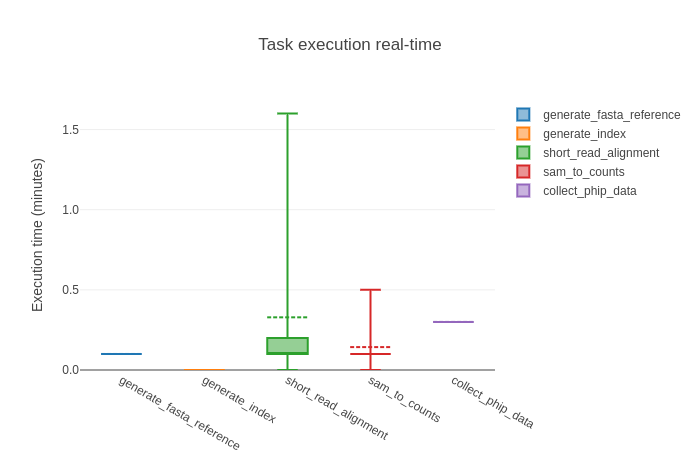
\includegraphics[width=.8\linewidth]{figures/time.png}  
  \caption{Distribution of total process execution time for each process definition}
  \label{fig:sub-first}
\end{subfigure}
\begin{subfigure}{.5\textwidth}
  \centering
  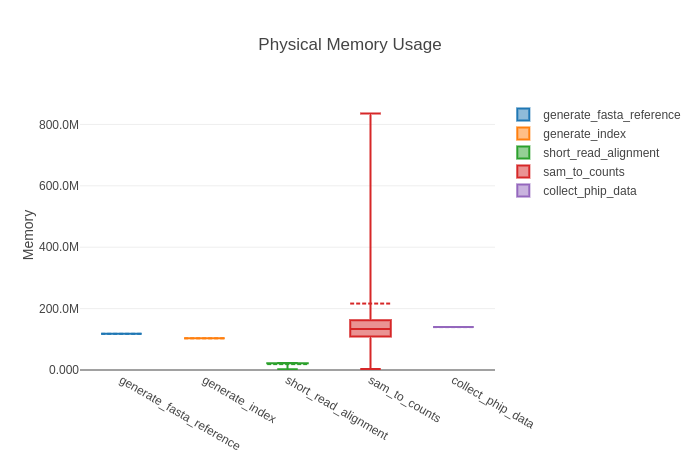
\includegraphics[width=.8\linewidth]{figures/memory.png}  
  \caption{Distribution of total process memory usage for each process definition}
  \label{fig:sub-second}
\end{subfigure}
\end{figure}

As a first look at the results, we can very easily plot the raw counts in the matrix as a heatmap.
Figure \ref{fig:raw_counts} shows this for our empirical dataset across 6 different individual sequencing experiments all included in the singular pipeline run.
It seems as though the experiments $1, 2$ and $4$ have consistent looking horizontal bands, where the others are quite noisy.
This pattern conforms to what we observe when plotting sample-specific technical replicate correlation in Figure \ref{fig:tech_reps}.
In other words, samples from experiments $3, 5$ and $6$ were not did not show reproducibility, and thus we can expect high quality results in the enrichment matrix.
The bars showing correlation for technical replicates are colored their factor status in one of the many sample metadata columns.

\begin{figure}[h!]
    \centering
    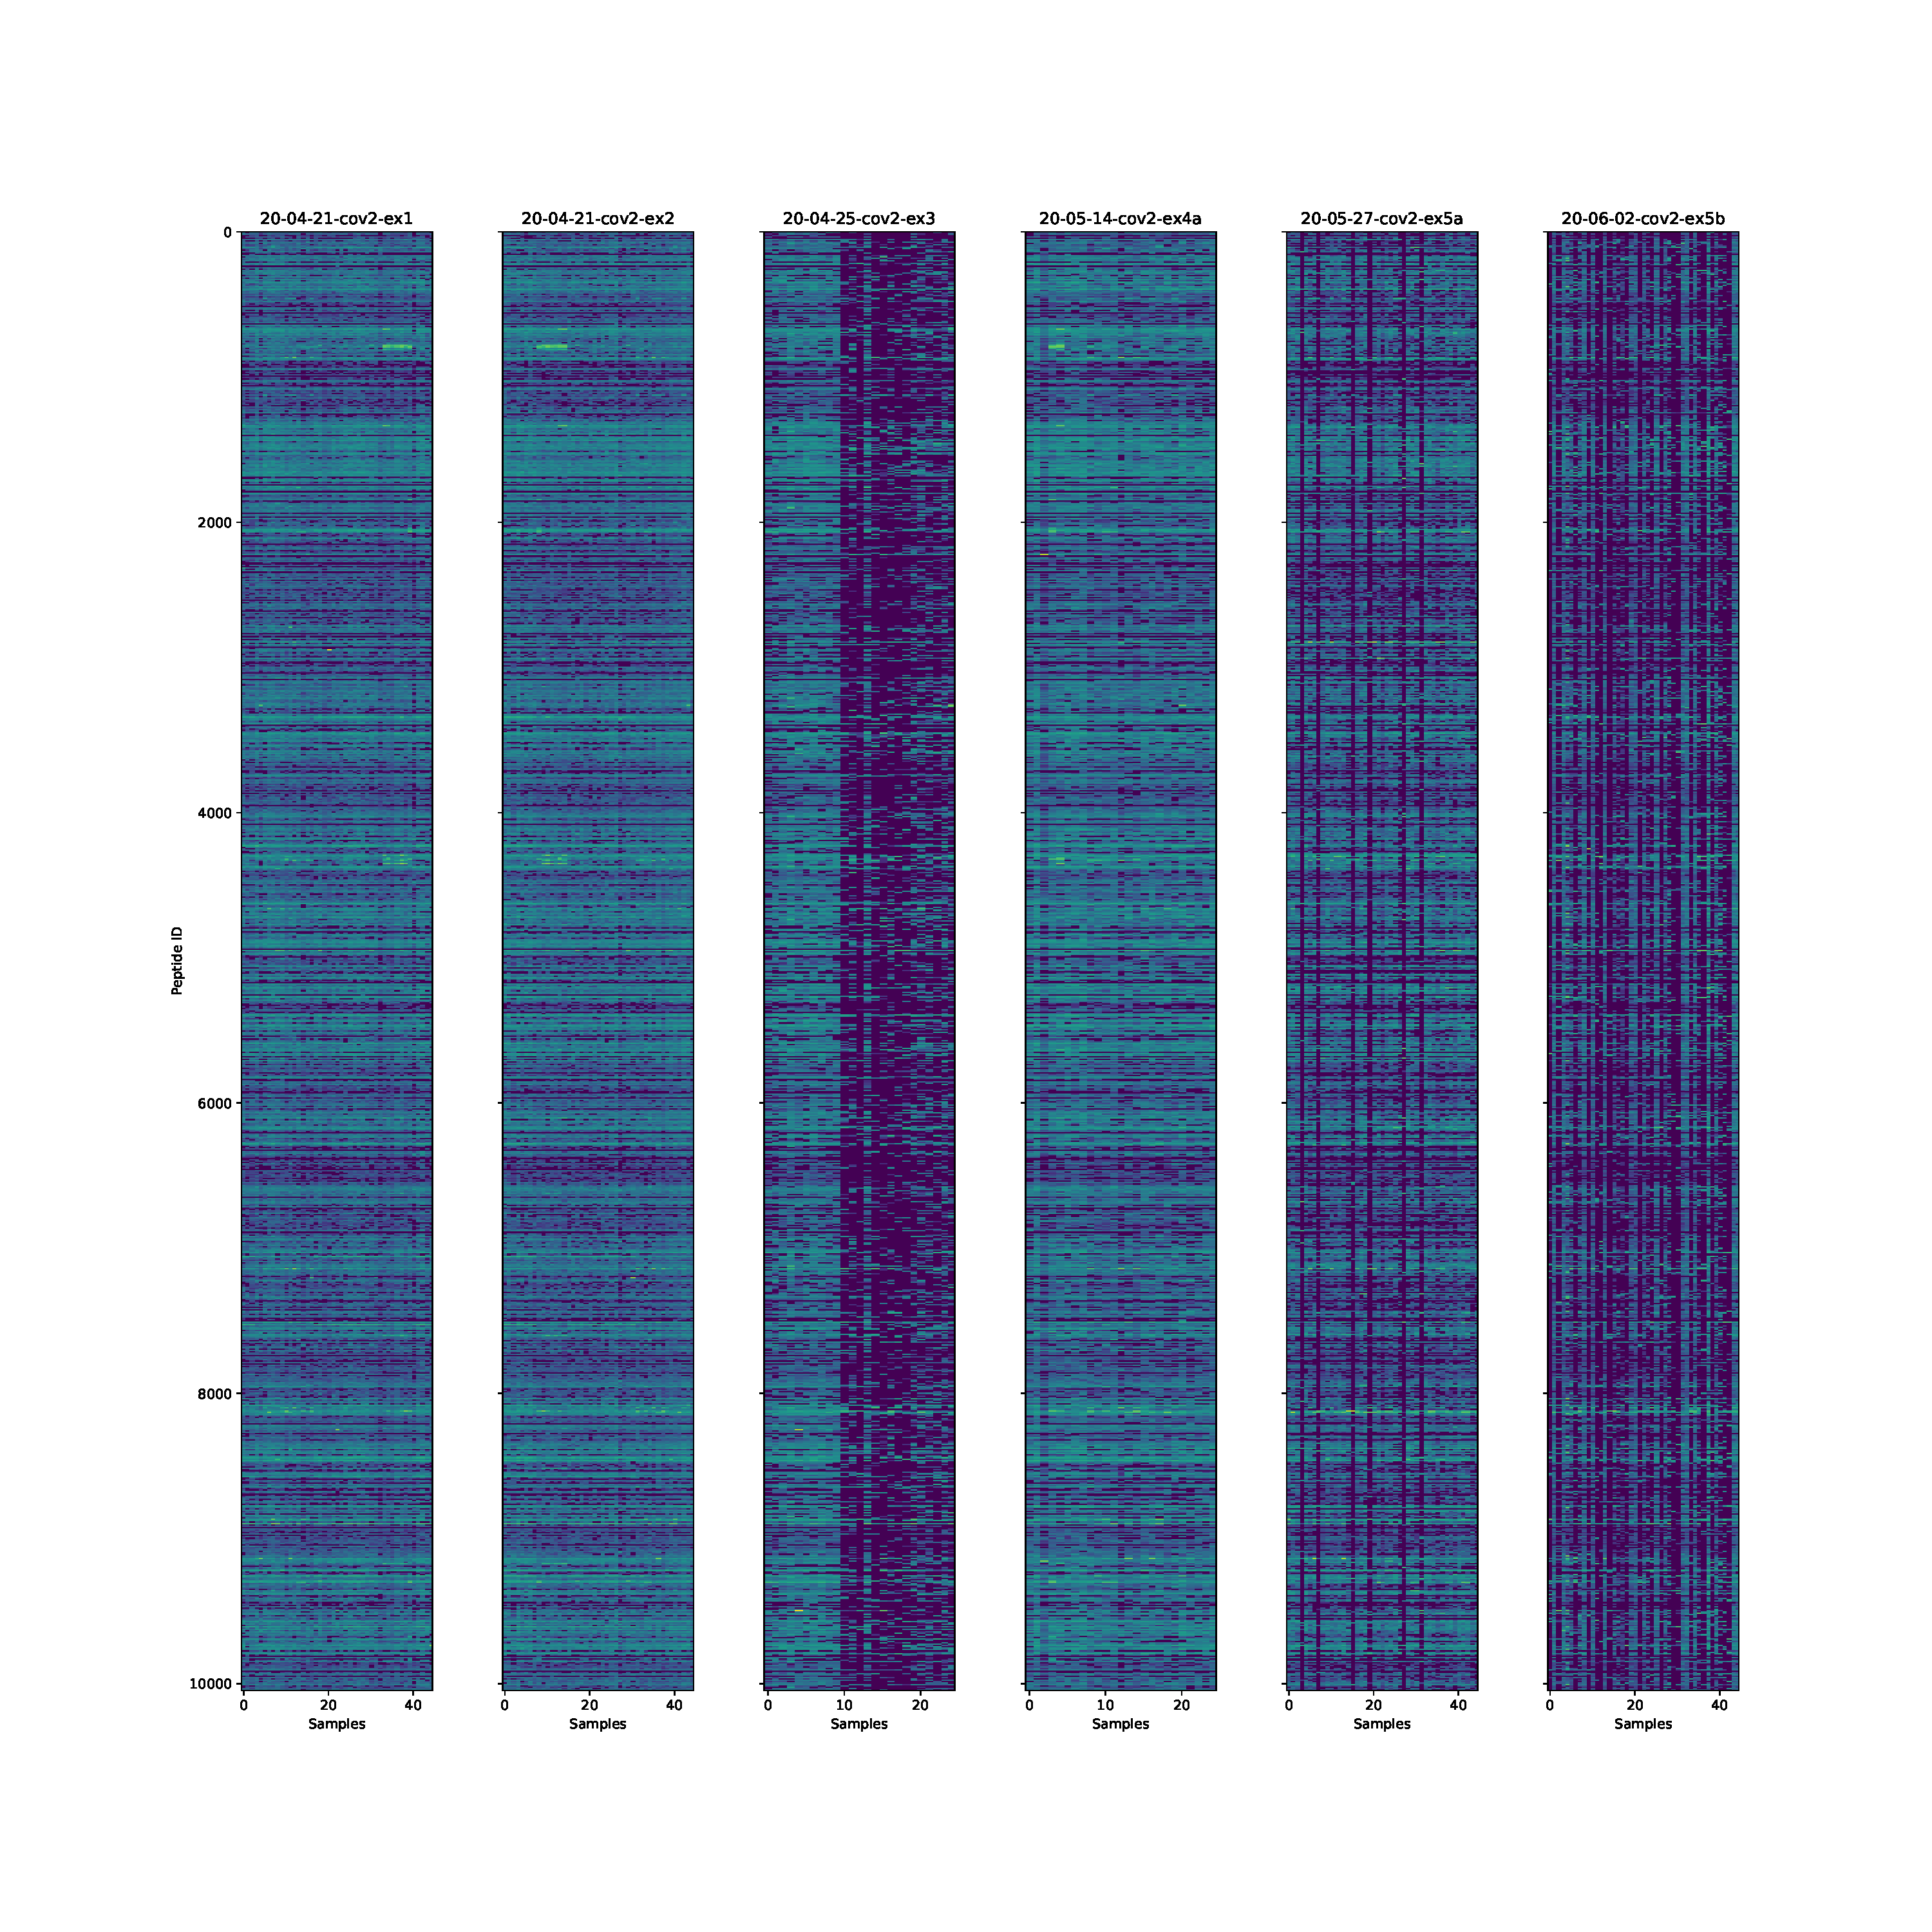
\includegraphics[width=1.0\textwidth]{figures/raw_counts.pdf}
    \caption{ \
    A heapmap showing the raw counts matrix, grouped by experiment.
    }
    \label{fig:raw_counts}
\end{figure}

Finally, in Figure \ref{fig:anon_all}, we show \textit{Standardized Enrichment} across all samples for a single experiment.
Concretely, this means we divide columns by the column sum to get sample specific enrichment \textit{frequencies} before dividing 
by a library input control and subtracting a ``beads-only" mock IP negative control.
We then group samples by a their respective status in another sample metadata columns to observe group differences as seen in Figure \ref{fig:anon_split}

\begin{figure}
\centering
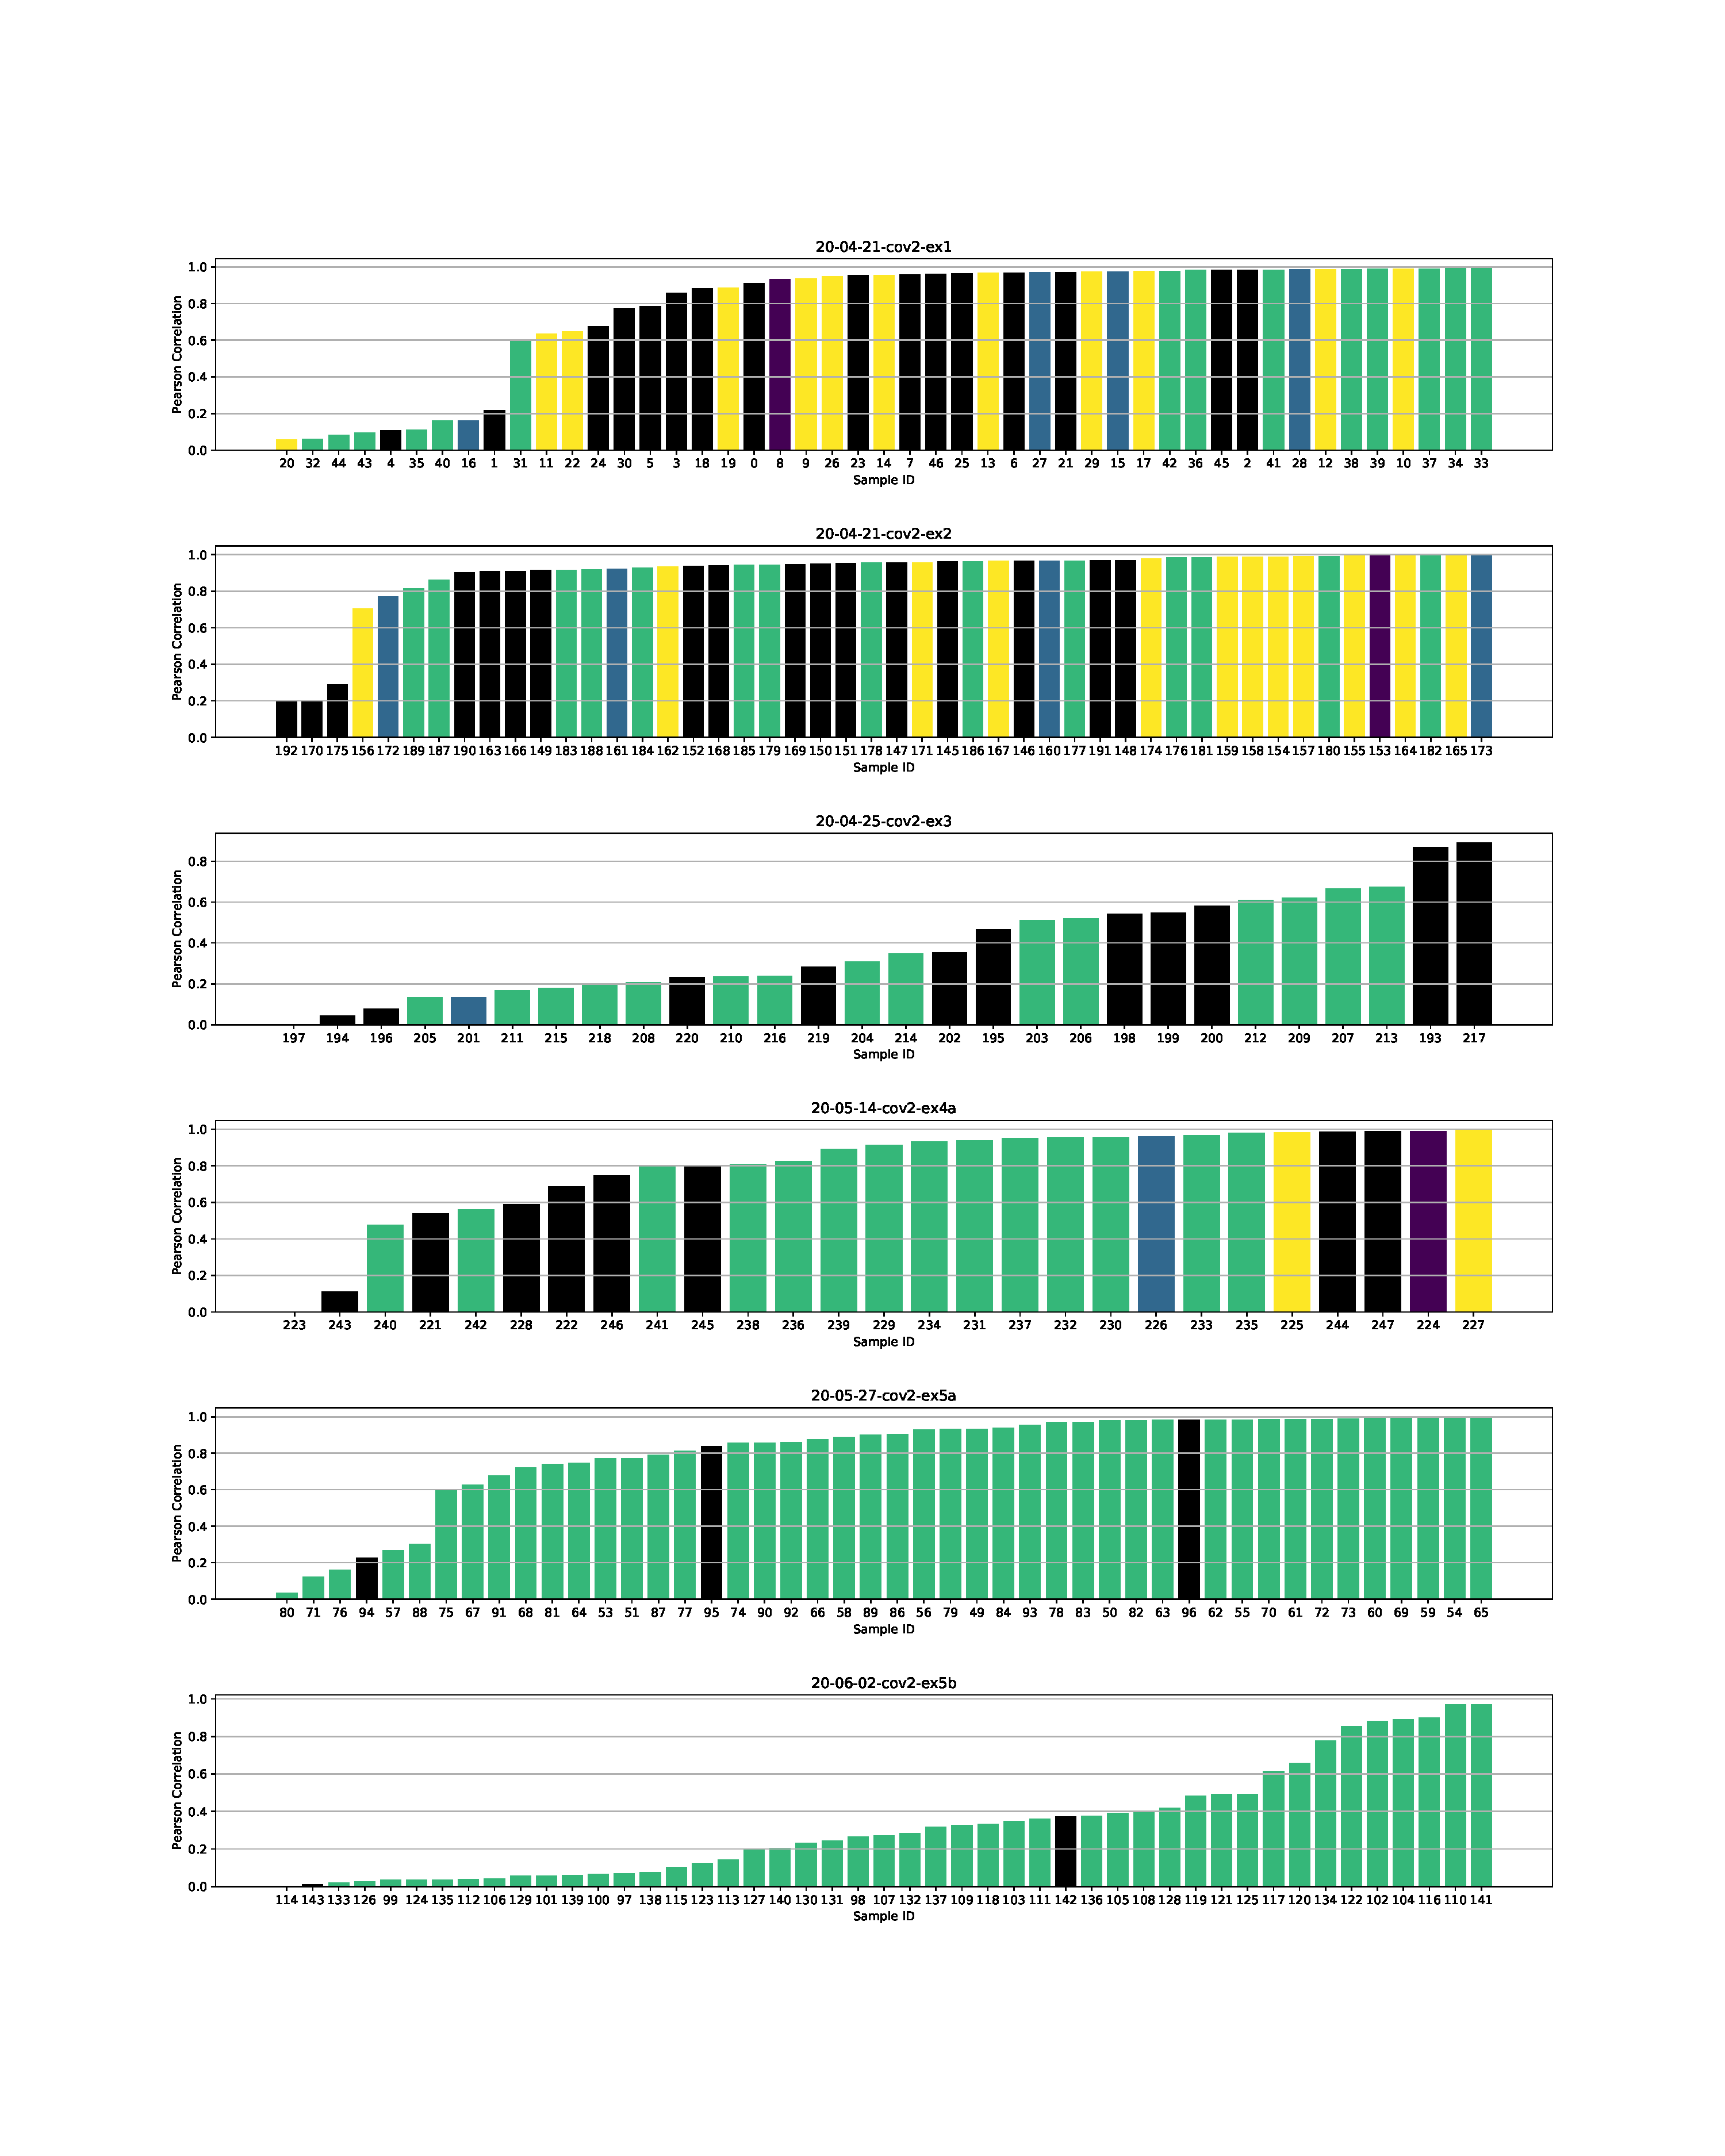
\includegraphics[width=1.0\textwidth]{figures/ANON_TECH_REP.pdf}
\caption{ \
Technical replicate correlation for each sample with greater than one replicate, grouped by experiment and colored by a sample metadata column.
}
\label{fig:tech_reps}
\end{figure}

\begin{figure}
\centering
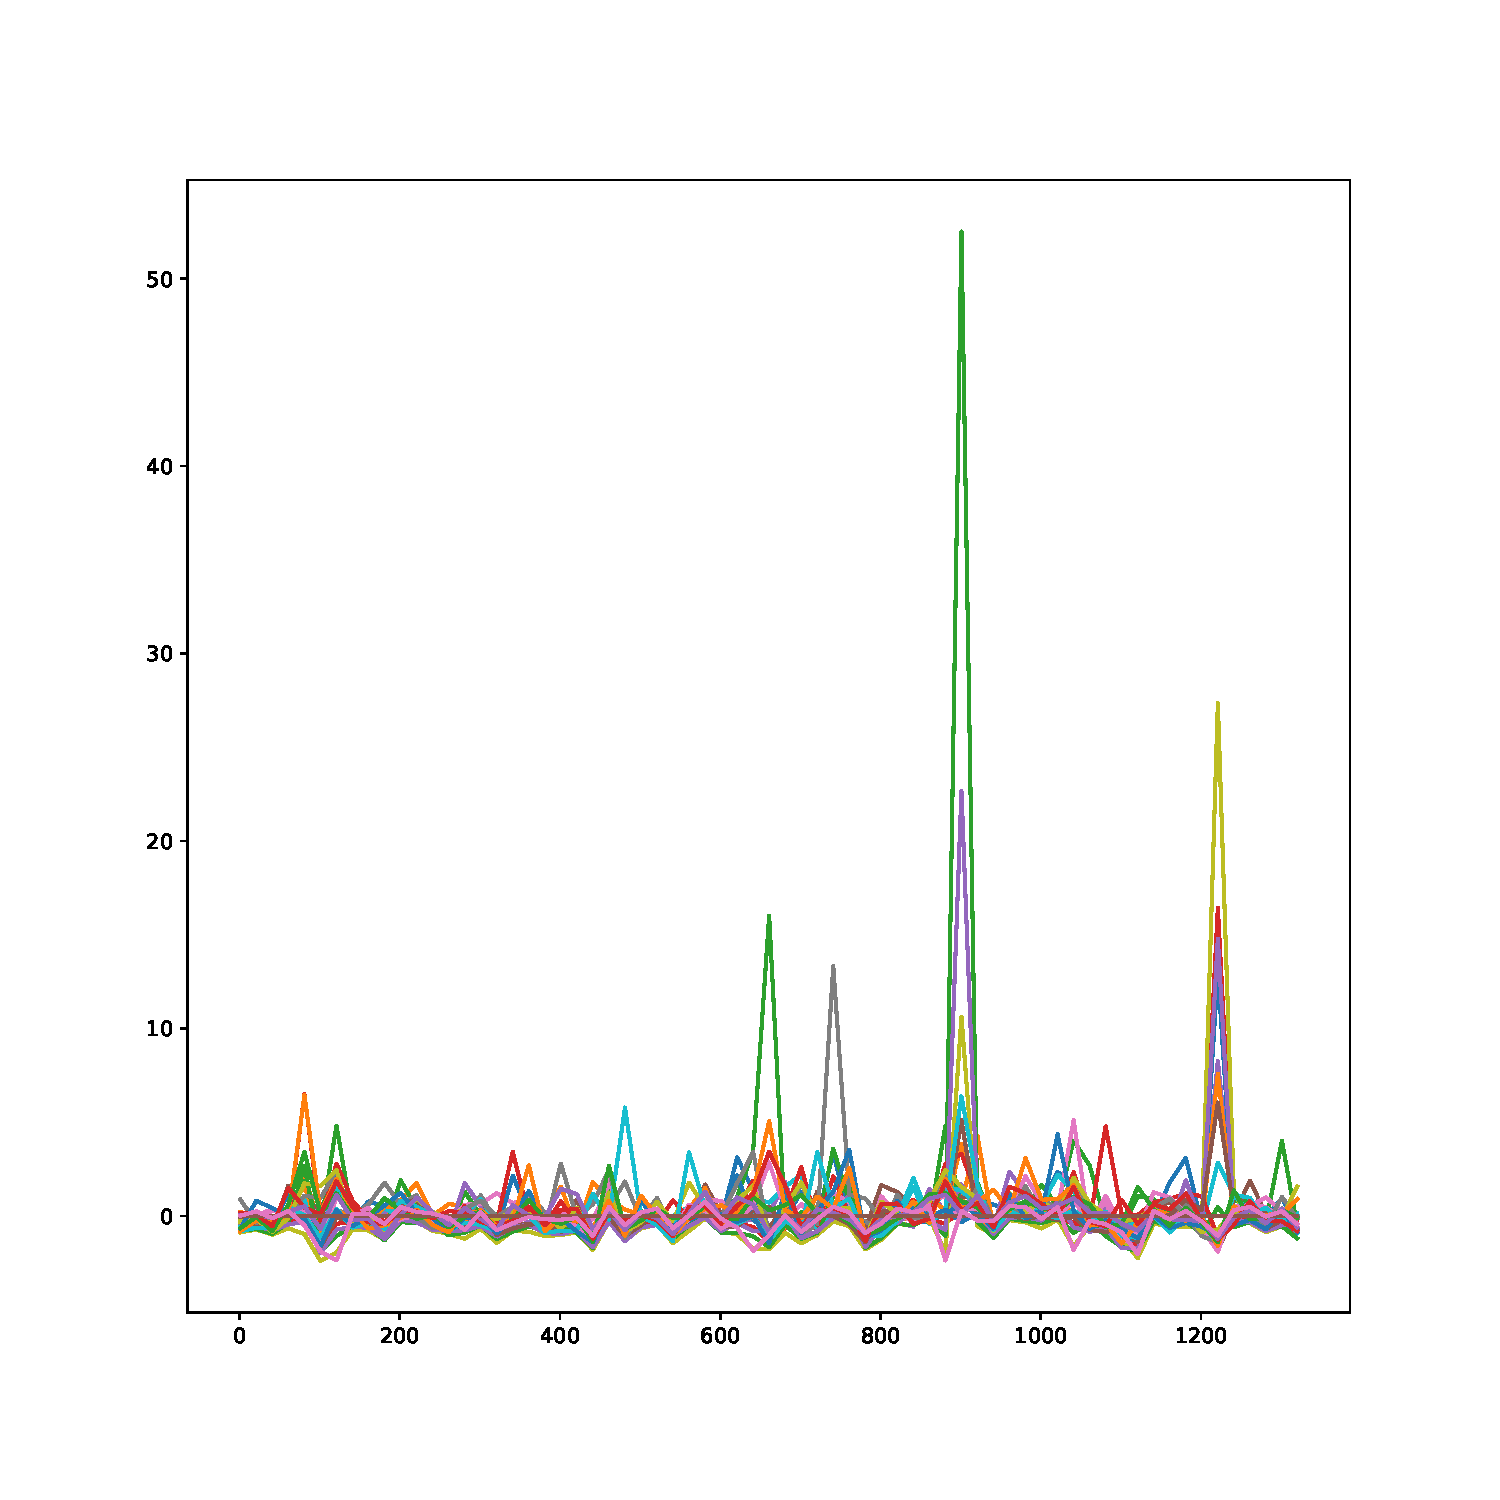
\includegraphics[width=1.0\textwidth]{figures/ANON_all_samples.pdf}
\caption{ \
Standardized enrichment for strain <X>, plotted as a function of tile genomic location. Each line represents a single samples enrichment.
}
\label{fig:anon_all}
\end{figure}



\begin{figure}
\centering
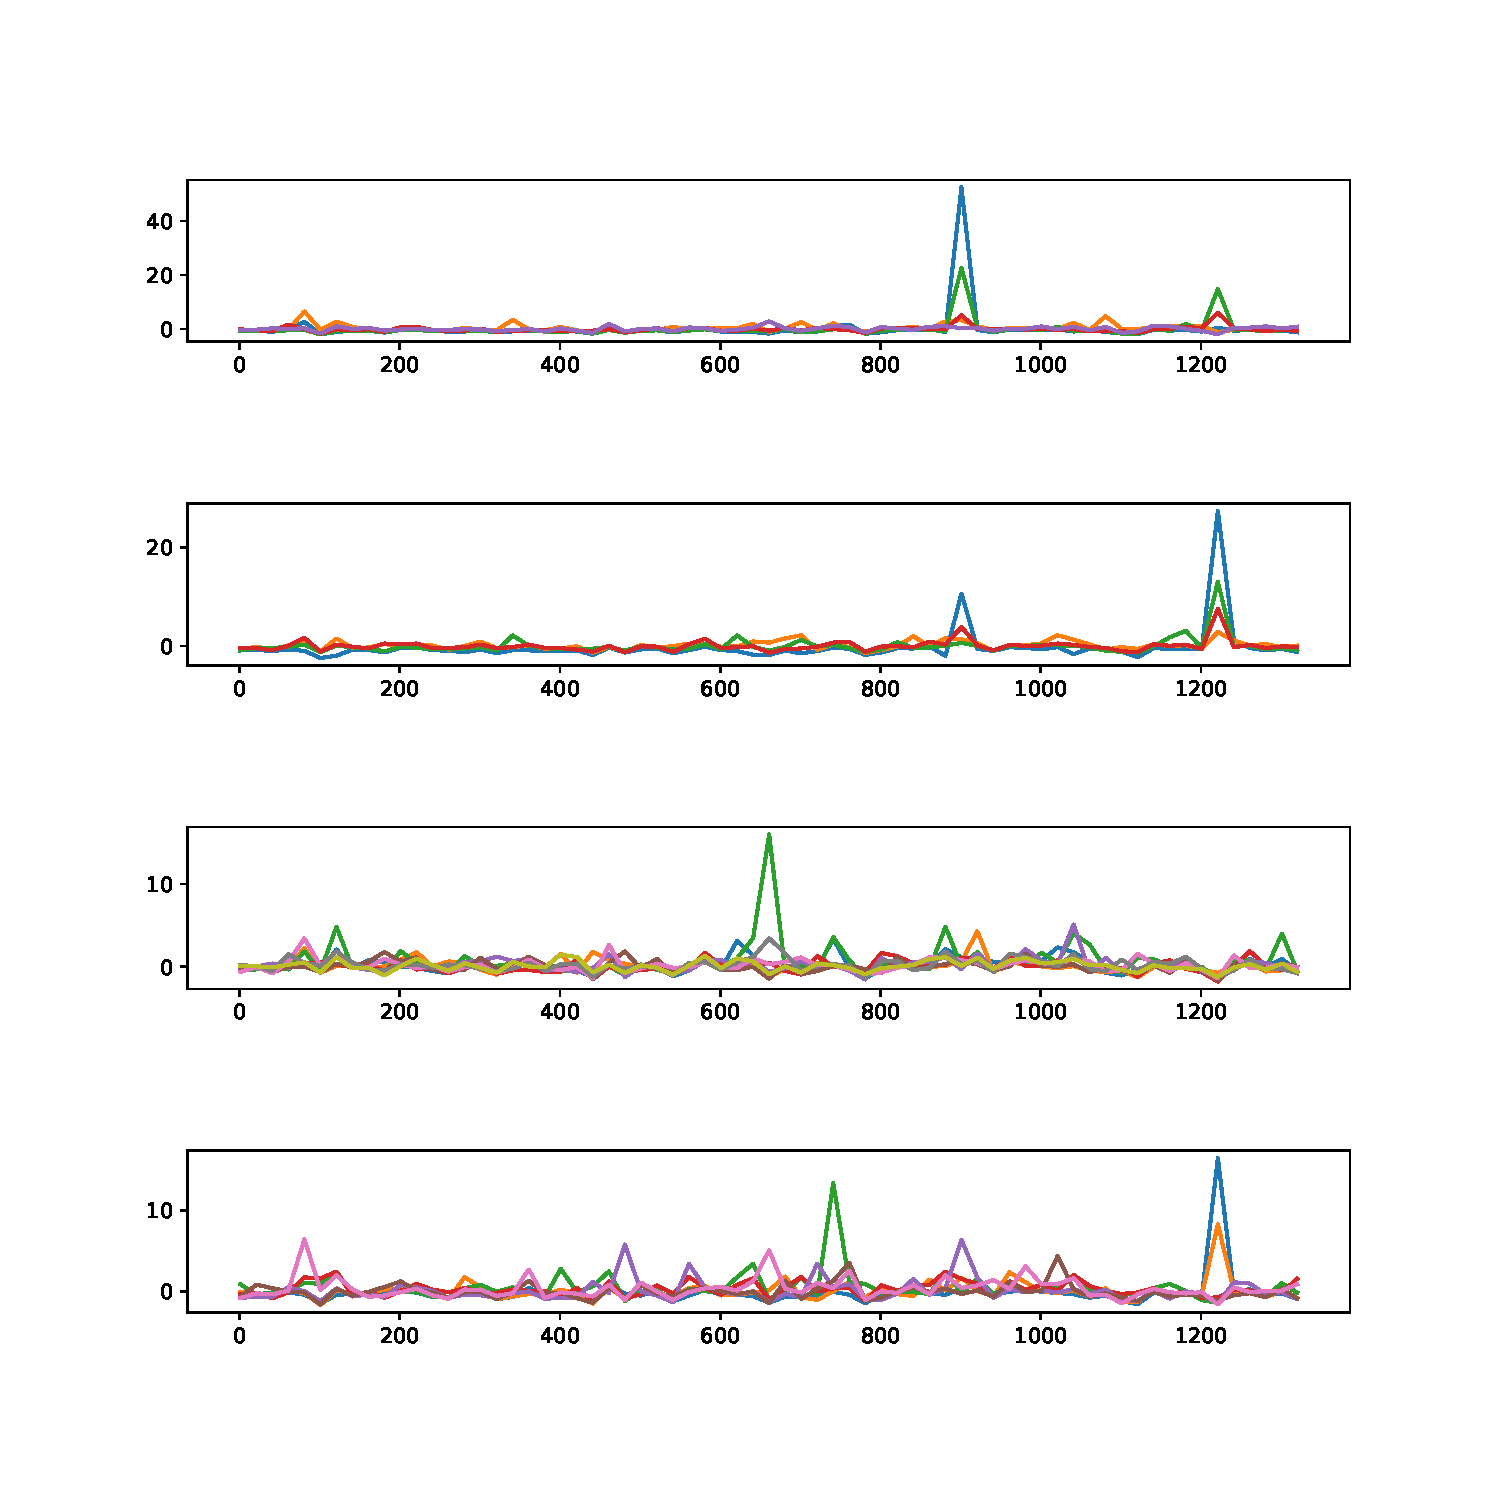
\includegraphics[width=1.0\textwidth]{figures/ANON_split.pdf}
\caption{ \
Standardized enrichment for strain <X>, plotted as a function of tile genomic location. The samples are then grouped by a column in the sample metadata column.
}
\label{fig:anon_split}
\end{figure}

\clearpage
\bibliographystyle{plain}
\bibliography{main}

% \clearpage
% \section*{Supplementary Materials}
% \beginsupplement
% Supplementary text and figures here.

\end{document}




